% #############################################################################
% This is Chapter 2
% !TEX root = ../main.tex
% #############################################################################
% Change the Name of the Chapter i the following line
\fancychapter{Related Work}
\cleardoublepage
% The following line allows to ref this chapter
\label{chapter:related-work}

\noindent During this chapter we will explore some concepts that are directly related to our work.
Firstly, we talk about how the game industry is making \acp{NPC}, and what are the key aspects for the creation of believable characters.
Then, we explore some of the existing frameworks and tools currently available for creating and testing agents for games, and multi-agents systems.
Afterwards, we move onto presenting and analyzing some agent's models and architectures.

\section{Games, Immersion and Believability}

\noindent As we argued before, the increasing lifelikeness in video games gives players increasing expectations of better, meaningful experiences and interactions.
The world around the player is presented with exquisite graphics and increasing levels of fidelity, as proved by the recent title from Guerrilla Games, Horizon Zero Dawn \cite{games:horizon} (Figure \ref{fig:horizon}).

However, \acp{NPC} still have a lot of room for improvement.
Scripted behaviour and repetitive dialog, products of the lack of socially deep \acp{NPC}, can easily break the gaming experience of the player, due to reduced believability in the \acp{NPC} actions \cite{thrainsson:emotion-games}.
This contrast between the world and it's inhabitants may break the suspension of disbelief, one of the major factors needed to achieve a successful gaming experience \cite{ijsselsteijn:userexperience}.

The concept of believable characters has long been studied and explored in many different forms of art and media \cite{bates:emotioninagents}.
From the original Disney animators of the 1930's and the book later published on Disney's animations \cite{illusionoflife}, we can understand that in order to have believable characters we need to create the illusion of life.

\begin{figure}
  \centering
  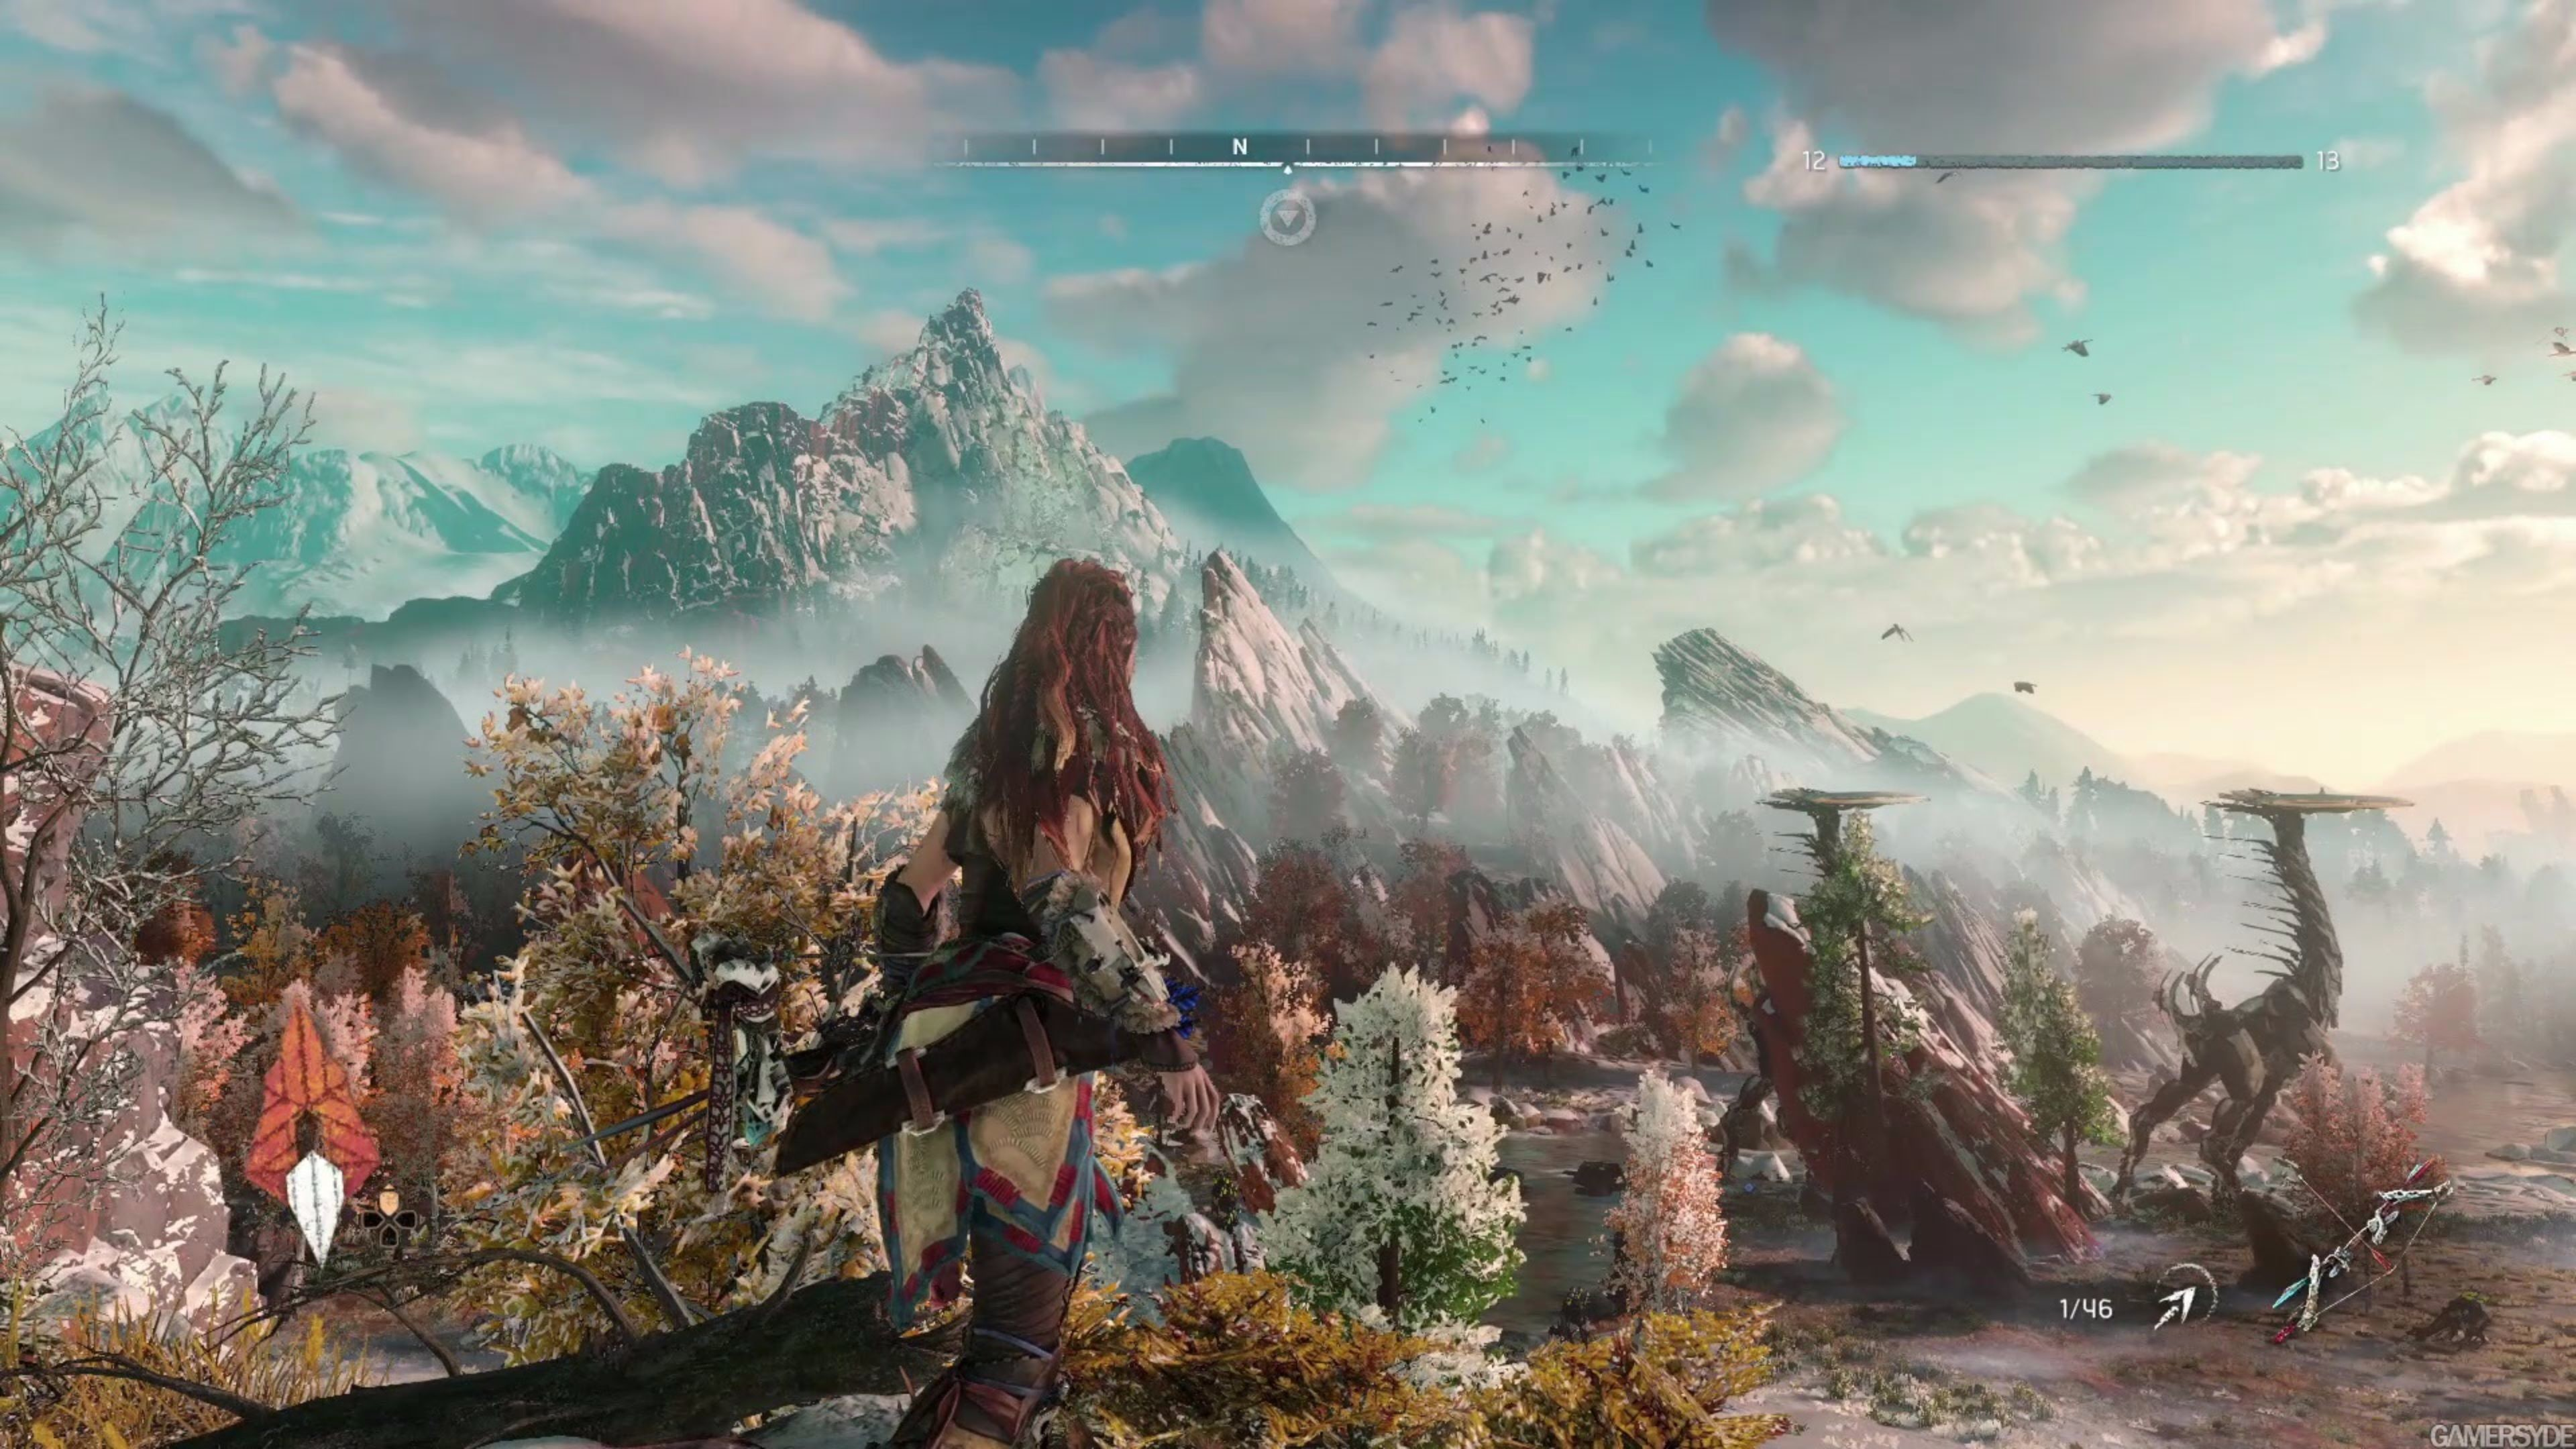
\includegraphics[width=\textwidth]{./Images/horizon-zero-dawn}
  \caption{Horizon Zero Dawn exquisite graphics.}
  \label{fig:horizon}
\end{figure}

\subsection{NPCs in games}

Most Triple-A video games make use of simple techniques to express \ac{NPC} behaviour.
Finite State Machines (FSM), hierarchical FSM and behaviors trees are the most commonly used techniques in nowadays industry \cite{yannakakis:gameairevisited}.
However simple, they can achieve believable and expressive behaviours in the hands of skilled game designers.
These techniques can express logic, basic planning and reactive behaviours.

Another advantage is that these techniques are deterministic, in other words, we can predict what can happen and then try to avoid problems.
Their major weakness, however, is their limited expressiveness, which can cause the realization of complex behaviors unmanageable.

In games like Assassin's Creed Unity \cite{games:assassinscreedunity} and Dragon Age Inquisition \cite{games:dragonageinquisition}, where there is a large number of \acp{NPC}, there is a tendency to make them reactive to the players instead of actively following their own goals.
In Dragon Age Inquisiton, many \acp{NPC} are present throughout the world doing absolutely nothing (check Figure \ref{fig:dragonage}).
Sometimes, when the player approaches, she can overhear a conversation that is taking place between \acp{NPC}, usually directly related to the player, but these are always simple one or two sentences conversations and the player cannot interact with the \ac{NPC} that is talking.

One can argue that, using current technology, it is impossible to make every single \ac{NPC} socially aware and able to interact with the player.
However, even if we only look at the \acp{NPC} with which we can interact, their behaviour is repetitive and lacks depth.

Other games, such as The Elder Scrolls V: Skyrim \cite{games:skyrim}, have \acp{NPC} with occupations which they carry out, during the day (the blacksmith will spend her day at the forge working), and houses where they return to, during the night (almost every character will go to his home to have a meal and sleep).
These simple behaviours highly contribute to the character's believability as it provides the sense of having wants and needs. However, they still lack social ability.

If, for example, the player breaks into the house of a random \ac{NPC}, wakes her up and has a talk with her, she will ignore the fact that you just woke her up in the middle of the night in her locked house and proceed to have a completely normal conversation with the player.
The weirder part still, is that the player will be branded as a criminal and may face the city's guards upon exiting the house.
This lack of social ability can easily break the player's suspension of disbelief.

To address this problem we can make use of research based agency models for \ac{NPC} control, as has been done in other works \cite{guimaraes:cif-ck-17}\cite{ferreira:merchant-model}.

\begin{figure}
  \centering
  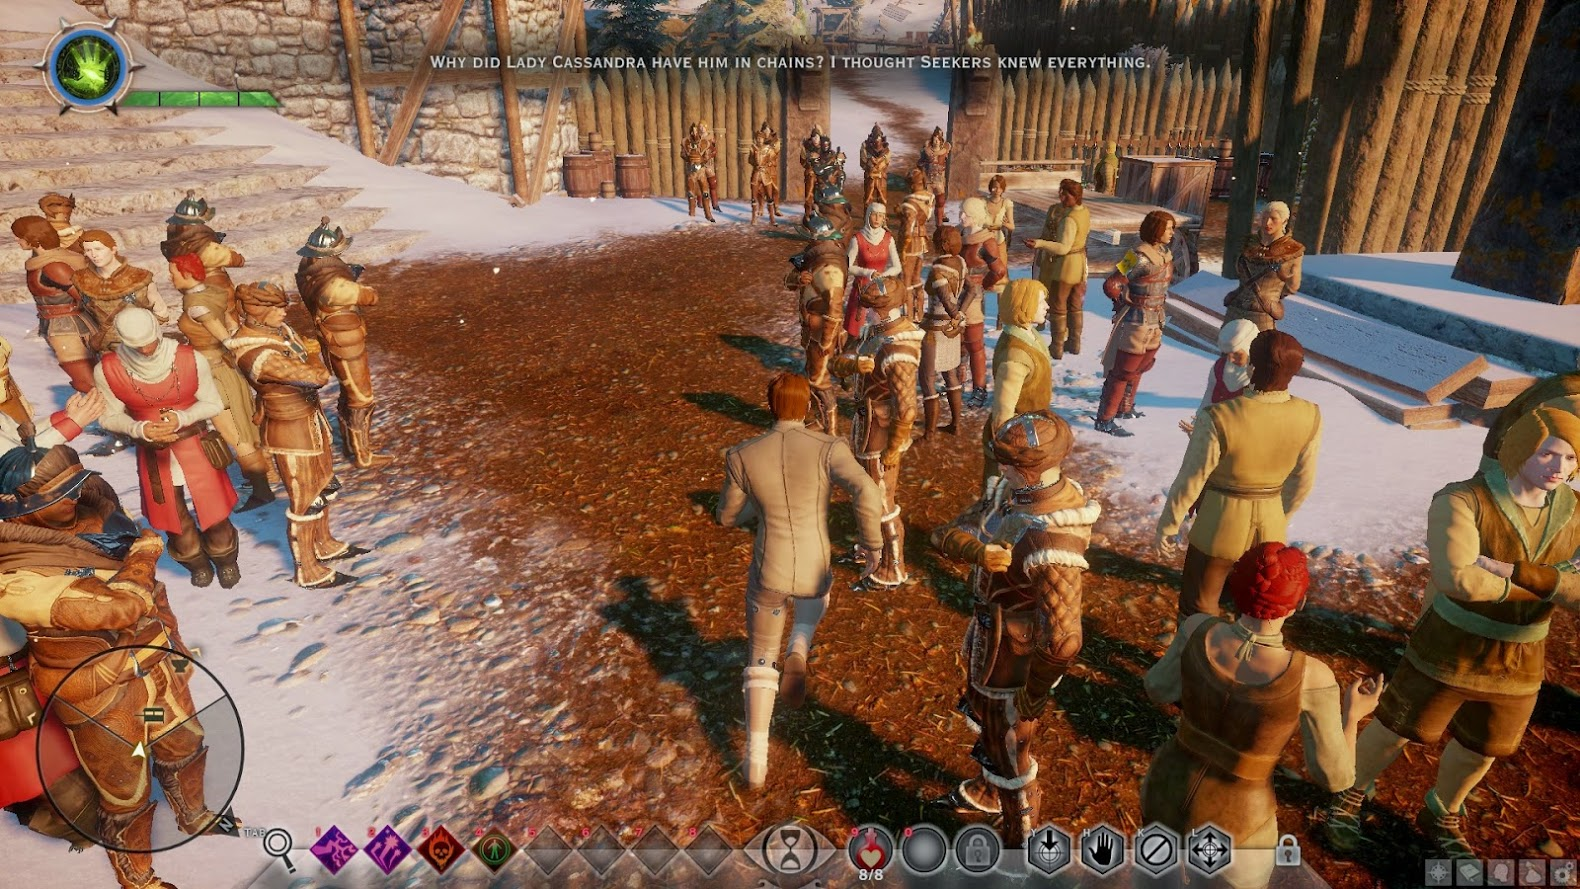
\includegraphics[width=\textwidth]{./Images/DragonAgeInquisition}
  \caption{Example of Dragon Age Inquisition's NPCs.}
  \label{fig:dragonage}
\end{figure}

\subsection{Socially empowered games}

\noindent There are, however, some examples of socially focused games that are worth to mention not only for their value as games but also for their successful use of research based agency models for \ac{NPC} control.

\subsubsection*{Blood and Laurels}
\label{subsection:bloodnlaurel}

Blood and Laurels (Figure \ref{fig:versu}) is a text-based interactive drama available in the App Store for the iPad\footnote{You can visit the game webpage at https://versu.com/2014/05/28/blood-laurels/.}.
One of the game's appeal is its high replayability due to the use of autonomous agents.
The same episode can be played several times with different results.
This is only made possible by making use of the Versu model \cite{evans:versu}, described in \ref{subsection:versu}.

\begin{figure}
  \centering
  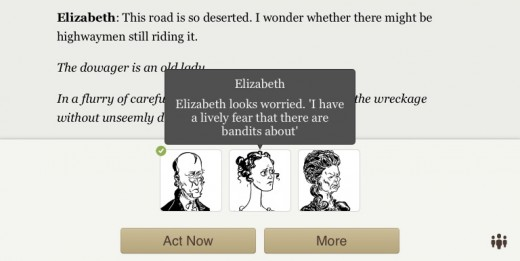
\includegraphics[width=0.7\textwidth]{./Images/versu}
  \caption{A screen shot of Blood and Laurels' game play.}
  \label{fig:versu}
\end{figure}

Blood and Laurels is set in ancient Rome and the player must weave through a web of conspiracies and politics.
The game's success and critics are proof that the use of socially aware \acp{NPC} can produce highly adaptable and interesting games.
The creators of Blood and Laurels are currently working on a second title called Bramble House which will also use Versu as the base for the autonomous characters (\acp{NPC}).

\subsubsection*{Prom Week}

\noindent Prom Week is a social simulation game about the interpersonal lives of a group of high school students in the  week leading up to their prom\cite{mccoy:prom-week}.
Gameplay in Prom Week involves solving level goals (such as making the class nerd, Zack, date a popular girl) within a limited number of turns by directing the characters to engage in social interactions.

What social games are available and how each changes the social state is managed by the game's \ac{AI} system, \ac{CiF}, described in \ref{subsection:cif}.
Enabled by the social physics of \ac{CiF}, each level's goal has innumerable solutions that maintain character believability.

\subsubsection*{Mismanor}

\noindent Mismanor is a social role-playing game where the player’s main form of interaction are actions that change the underlying social model \cite{sullivan:mismanor}.
It makes use of an adaptation of the \ac{CiF} architecture discussed in \ref{subsection:cif}.
In Mismanor, the player is guided through the dynamic story with quests that are chosen based on the actions the player has taken and their social standing with the character they are interacting with.
Quests have multiple entry and exit points, giving the player more flexibility with how they choose to fulfill the request, with different consequences based on the path they have taken.

\subsubsection*{Façade}

\begin{figure}
  \centering
  
\includegraphics[width=0.7\textwidth]{./Images/facade-screenshot}
  \caption{The two NPCs of Façade greeting the player as she arrives at the dinner party.}
  \label{fig:facade}
\end{figure}

\noindent In Façade\cite{mateas:facade}, the player is given almost no direction or role to play.
The player can either play herself as the character or interpret the part of whomever she wishes.
The drama takes place in a small simulated virtual world, the apartment of the married couple Grace and Trip.
Façade was designed to deliver an experience that provides the player with 20 minutes of emotionally intense, undefined, dramatic action.
The player's actions have a significant influence on how the story develops and how the drama ends.

% \subsection{Research on Game AI}

% In Guimarães' work \cite{guimaraes:cif-ck}, \ac{NPC}s have social desires and complex behaviours and work towards changing the social state around them.
% The player can see them in action and decide whether or not he/she will interfere, introducing another kind of decision making in the game, one with immediate and visible consequences.

\section{Tools and Frameworks}

\noindent During this section we'll talk about some of the frameworks and tools currently available for the creation of agents.
We'll begin by presenting the well known Java framework \ac{JADE} and the \ac{FIPA} specification which \ac{JADE} is based upon.
Then, we'll talk of NetLogo and finally we'll present the PsychSim tool.

It is important to note that, to the best of our knowledge, there is, currently, no tool or framework that focuses in the development of \acp{NPC} for survival games.

\subsection{JADE}

\noindent \ac{JADE} is a software framework in compliance with the \ac{FIPA} specifications for interoperable intelligent multi-agent systems made in Java \cite{bellifemine:jade}.
It aims to simplify the development of agents while maintaining standard compliance through a comprehensive set of system services and agents.
\ac{JADE} complies with \ac{FIPA}'s specification \cite{obrien:FIPA} which defines the rules that allow a society of agents to operate, inter-operate, and be managed. This specification is further detailed bellow, in \ref{subsubsection:FIPA}.

While complying with the \ac{FIPA} specification, \ac{JADE} provides a set of abstractions that allow for the rapid development of agents, like the use of an abstraction model called Behaviour. 
Behaviours model the tasks that an agent is able to perform and each agent instantiates their behaviours according to their needs and desired capabilities.
The framework also includes some ready to use behaviours for the most common tasks in agent programming, such as sending and receiving messages and structuring complex tasks as aggregations of simpler ones.
The developer needs only to extend the Agent class and implement the agent-specific tasks through one or more Behaviour classes, instantiate them, and add the desired behaviours to the agent.

\subsubsection*{FIPA}
\label{subsubsection:FIPA}

\noindent The \ac{FIPA} specifications represent the first step towards an agent standard \cite{obrien:FIPA}.
The specification does not attempt to define the internal architecture of agents nor how they should be implemented, but they do specify the interfaces necessary to support interoperability between agent systems.
It identifies the roles of some key agents necessary for the management of the platform, and specifies the agent management content language, ontology, and agent communication.

Three key roles are identified as mandatory in an agent platform.
The Agent Management System is the agent that exerts supervisory control over access to and use of the  platform; it is responsible for authentication of resident agents and control of registrations.
The Agent Communication Channel is the agent that provides the path for basic contact between agents inside and outside the platform; it is the default communication method which offers a reliable, orderly and accurate message routine service.
The Directory Facilitator is the agent that provides a yellow page service to the agent platform.
Notice that no restriction is given to the actual technology used for the platform implementation: e-mail based platform, Java applications, web services... these could all be FIPA compliant implementations.

Agent communication is based on message exchange, where agents communicate by formulating and sending individual messages to each other.
The \ac{FIPA} \ac{ACL} specifies a standard message language by setting out the encoding, semantics and pragmatics of the messages.
The standard does not set out a specific mechanism for the internal transportation of messages.
Instead, since different agents might run on different platforms and use different networking technologies, \ac{FIPA} specifies that the messages  transported  between  platforms  should  be  encoded  in  a  textual  form.

Other  parts  of  the  \ac{FIPA}  standard  specifies  other  aspects,  in  particular  the  agent-software
integration, agent mobility and security, ontology service, and the Human-Agent Communication.

\subsection{NetLogo}

\noindent NetLogo (Figure \ref{fig:netlogo}) is a multi-agent programming language and modeling environment for simulating natural and social phenomena \cite{tisue:netlogo}.
Modelers can give instructions to hundreds or thousands of independent agents, called ``turtles".
These turtles can represent molecules, animals, people, bacteria, cars, robots, neutrons, magnets, planets, or whatever the modeler decides.
The turtles move across a grid of ``patches" which are also programmable agents.
All of the agents can interact with each other and perform multiple tasks concurrently.
This makes it possible to explore connections between micro-level behaviors of individuals and macro-level patterns that emerge from their interactions.

NetLogo comes with a Models Library, which contains several simulations.
This collection has more than 140 pre-built simulations that can be explored and modified.
These simulations address many areas in the natural and social sciences, including biology and medicine, physics and chemistry, mathematics and computer science, and economics and social psychology.

\begin{figure}
  \centering
  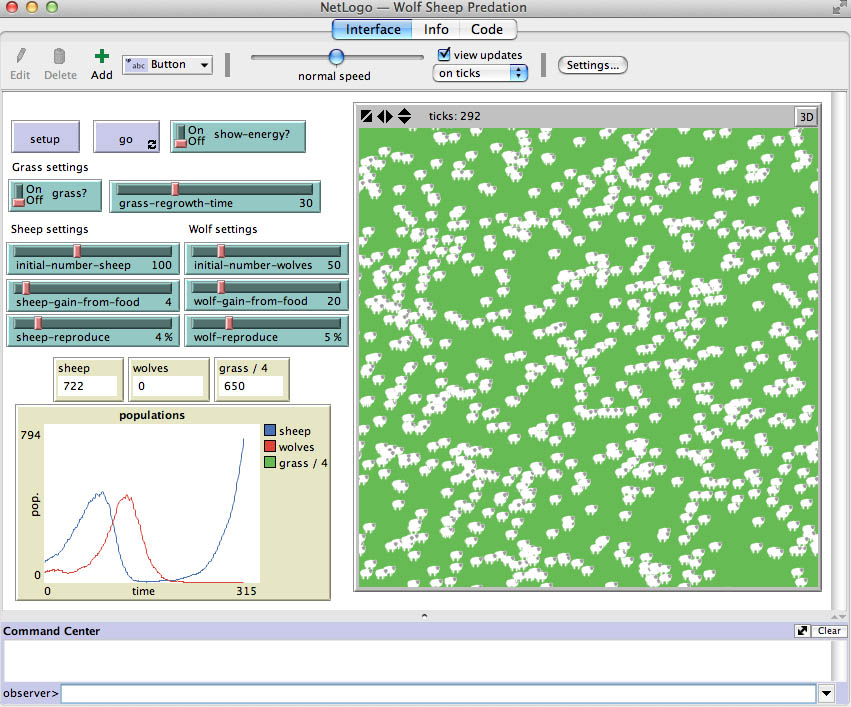
\includegraphics[width=0.7\textwidth]{./Images/netlogo5}
  \caption{NetLogo's interface.}
  \label{fig:netlogo}
\end{figure}

\subsection{PsychSim}
\label{subsection:psychsim}

\noindent PsychSim \cite{marsella:psychsim} is a social simulation tool developed to explore how individuals and groups interact and how can these interactions be influenced.
The work's foundation is the fact that social interactions are based on beliefs about other's minds, a \textit{theory of mind} \cite{whiten:theoryofmind}.
Psychsim allows developers to author and explore a social scenario of their creation through the selection of generic agents models and its further specialization, see Figure \ref{fig:psychsim}.
This tool allows developers to try and understand how a specific social group might react to certain situations.

\begin{figure}
  \centering
  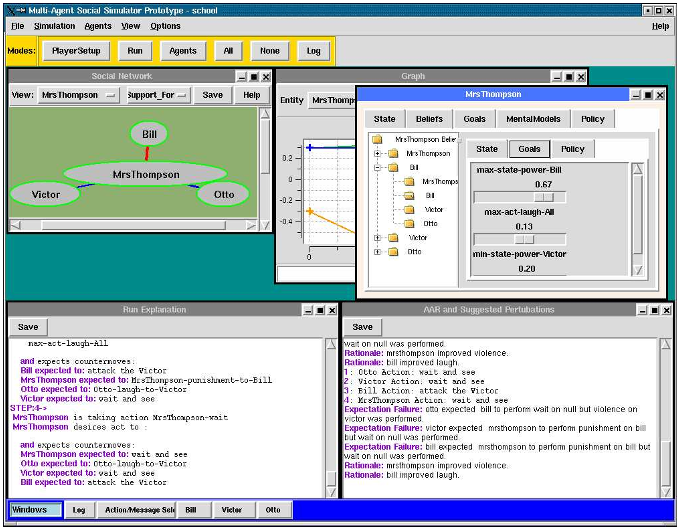
\includegraphics[width=0.7\textwidth]{./Images/psychsim}
  \caption{PsychSim tool for generating new scenarios and agents.}
  \label{fig:psychsim}
\end{figure}

PsychSim then simulates the behaviour for each entity, individual agent or group of agents, based on their preferences, relationships, private beliefs, and mental models about each other.

In the given example, the authors explore a bullying scenario in a school and try to answer several questions:
``\textit{How might a bully respond to admonishments, appeals to kindness or punishment? 
How might other groups react in turn? 
What are the predictions or unintended side effects?}".
The simulation tool then provides explanations of the results based on each entity's preferences and beliefs, allowing the authors to answer the previous questions.

PsychSim's agents are empowered with fully specified models of each other \cite{pynadath:modellingtheoryofmind}, a unique aspect of its design. Every agents maintains independent beliefs about the world, has its own goals, and it owns policies to achieve those goals. The model is composed by the state, actions, goals, beliefs, policies, messages, and mental models.

\begin{description}
\item \textbf{State} Each agent model includes a state with facts about the world, some of which may be hidden from the agent.
\item \textbf{Actions} Agents have a set of actions they can perform. Each action consists in an action type, a performer, and possibly an object of the action.
\item \textbf{Goals} These represent an agent's incentives for behaviours. In PsychSim, goals are reward functions that map the current state to a real value.
\item \textbf{Beliefs} The simulations agent have only a \textit{subjective} view of the world, where they form beliefs about what \textit{they} think is the state of the world. An agent's beliefs consists in models of all agents (including himself), representing their state, beliefs, goals, and policy of behaviour.
\item \textbf{Policies} Each agent's policy is a function that represents the process by which it selects an action or message based on its beliefs and goals.
\item \textbf{Messages} Messages are attempts by one agent to influence the beliefs of recipients and have five components: a source, recipients, a message subject, content, and overhearers.
\item \textbf{Mental Models} An agent's beliefs about another agent are realized as a fully specified agent model of the other agent, including goals, beliefs, and policies. Mental Models are predefined models which represent an agent's goals, beliefs, and policies.
\end{description}

\section{Social Architectures and Models}

\noindent In this section we take a look into existing models for agency.

\subsection{Comme il Faut and Ensemble}
\label{subsection:cif}
\noindent \ac{CiF} is an \ac{AI} system that enables authors to create interactive stories by specifying, not the complete narrative and all its ramifications but, high-level rules governing expected character behaviour given social situations \cite{mccoy:cif-social-story-worlds}.
In \ac{CiF}, characters use many attributes of the current social state, including the story of prior interactions, to decide how to engage in social exchanges with other characters.
This architecture provides a rich social environment for characters to interact allowing the creation of dynamic and interactive stories.

%\ac{CiF} does not store world information in a series of events, like many \ac{AI} techniques do (e.g. Behaviour Trees and Hierarchical Task Networks).
Social exchanges are the primary structure of representing knowledge in \ac{CiF} \cite{mccoy:cif-authoring}.
They consist in social interactions between characters that modify the social state of the participants.
By using social exchanges and additional encoded social context, \ac{CiF} lowers the authoring burden needed to create the social aspects of an interactive story by allowing the author to specify the rules and general patterns of how social interaction should take place.

Characters' behaviour is chosen based on rules in a large rule database that depict normal social behaviour in a particular story world.
These rules, in conjunction with the logic of a social world, a set of characters, and a series of scenario goals allows \ac{CiF} to determine the desired action for each character.

More recently, a new version of \ac{CiF} as been published and renamed to Ensemble.
Ensemble aims to empower \acp{NPC} with deeper interactivity and believability by modeling social states and behaviours for game characters \cite{treanor:ensemble}.
This extension presents a model of playable social dialogue called social practices.
Social practices increase the playability of character interactions and add interactivity at each stage of dialogue.

\subsection{Versu}
\label{subsection:versu}

\noindent Versu model is based on Exclusion Logic \cite{evans:exclusion-logic}, a new deontic logic, and rests upon two kinds of objects: agents and social practices.
To better make use of exclusion logic, the creators of Versu have also developed Praxis, a \ac{DSL} used in the modeling of the social practices .

Social practices describe a recurring social situation that may exist only for a short time (e.g. a conversation, a game, a meal) or can last much longer (e.g. a family, the moral community).
These practices coordinate agents via the \textit{roles} they are playing and their main function is to describe the actions the agents can do in each situation.

Social practices provide the agent with a set of suggested actions, but it is up to the agent to decide which action to perform, using utility-based reactive action selection (the utility is calculated in accordance with the agents beliefs, desires, personality quirks, and backstory).

Multiple practices can exist concurrently, for example, in a dinner party, there will be multiple practices operating at once:

\begin{itemize}
\item eating and drinking.
\item the conversation about politics
\item the rising flirtation between Frank and Lucy
\item responding to the fact that Mr. Quinn has spilled the soup.
\end{itemize}

Performing an action can result in any sentence being added to the world database.
The results of adding new sentences can be that relationships are updated, new beliefs or desires are formed, old practices are deleted or new practices are spawned.
Agents and social practices are scripts authored using the \ac{DSL} Praxis.

\subsection{FAtiMA}
\label{subsection:fatima}

\noindent \ac{FAtiMA} is an agent architecture with planning capabilities designed to use emotions and personality to influence the agent's behaviour \cite{dias:fatima-modular}.
The acronym stands for Fearnot AffecTIve Mind Architecture as it was developed to endow the characters in the serious game \textit{FearNot!} \cite{aylett:fearnot} with social intelligence.
It has been used successfully in different social scenarios (\cite{paiva:learning-by-feeling},\cite{rodrigues:i-can-feel-to}, \cite{aylett:intercultural-empathy}, and \cite{correia:sueca}) and it is based on appraisal theory \footnote{The theory that emotions are elicited by evaluations (appraisals) of events and situations \cite{roseman:appraisal}.}.

\ac{FAtiMA} has a modular architecture where functionalities and processes are divided into modular independent assets.
This enables developers to use a lighter and simpler version of \ac{FAtiMA} by adding the required assets, according to their necessities.
Therefore, behaviour and functionality are added by including assets in an agent's definition.
These assets will then implement the desired behaviours and functionalities.

\ac{FAtiMA} comes with a set of predefined assets that can be used to define agents and their interactions\footnote{The toolkit is available at https://github.com/GAIPS-INESC-ID/FAtiMA-Toolkit.}.
Additionally, the developer can create its own assets that extend the toolkit's capabilities.
The available assets are:

\begin{figure}
  \centering
  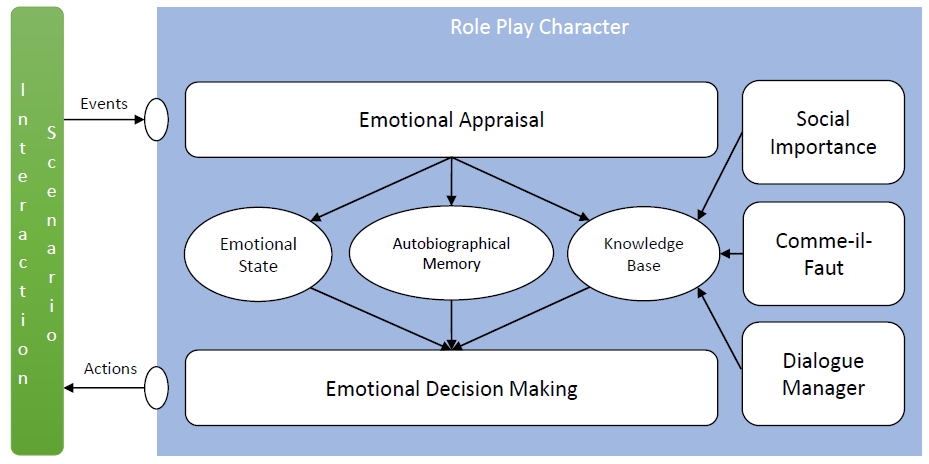
\includegraphics[width=\textwidth]{./Images/rpc}
  \caption{The Role Play Character Asset aggregating all other assets to make an autonomous agent.}
  \label{fig:rpc}
\end{figure}

\begin{description}
\item [Role Play Character Asset] \hfill

The \ac{RPC} Asset is an aggregation asset responsible for managing all the other assets that compose an agent.
It is also responsible for maintaining the agent's Emotional State and the agent's memory, which is divided in two components: a Knowledge Base and an Autobiographic Memory.

The Emotional State stores the current emotional state of the agent, defined by the Emotional Appraisal Asset, the Knowledge base stores the agent's beliefs, and the Autobiographic Memory stores the agent's recollections of past events and the emotions associated with such events.

Events are divided into three categories: Action-Start, Action-End, and Property-Change. The first two are self-explanatory and the third represents updates to the \ac{RPC}'s Knowledge Base.
Therefore, in order to update the Knowledge Base, the \ac{RPC} must perceive the appropriate events.

For consistency sake, both beliefs and events are described by \ac{WFN}.
These can be symbols (e.g. ``\texttt{Walter}" or ``\texttt{cutgrass}"), variables (e.g. ``\texttt{[x]}" or ``\texttt{[target]}"), and composed names (e.g. ``\texttt{IsBusy(Walter)}" or ``\texttt{Likes(Walter, [target])}").

\item [Emotional Appraisal Asset] \hfill

This asset appraises each event according to the OCC Theory of Emotions \cite{ortony:occ}.
Developer defined appraisal rules, determine how an agent evaluates certain events, determining the agent's Emotional State (which is kept by the \ac{RPC}).

For example, an agent, Mary, who likes John, might perceive the event of John flirting with her in a positive way, whilst another agent, Kate, who dislikes John, might perceive such flirtation negatively.

\item [Emotional Decision Making Asset] \hfill

The Emotional Decision Making Asset provides \acp{RPC} with decision making capabilities based on rules with logical conditions.
Allowing the agent to make multiple decisions at the same time, this asset makes use of the Knowledge Base and the Emotional State to decide which actions it decides to do.

The possibility of making multiple decisions at the same time is particularly interesting when considering behaviour related decisions and non-behaviour related decisions (dialogue actions and/or emotional responses).
\ac{FAtiMA} Toolkit handles this by making use of what it calls layers of decisions.
When the decision process is triggered, if a layer is provided, only actions for that layer are considered.

Additionally, this asset adds Dynamic Properties that can be used as conditions to actions.
Dynamic Properties provide a facility for developers to implement additional processing capabilities for the decision of certain actions.
For example, the developer could implement a \textit{Gaze} Dynamic property that would connect to an external eye tracking device, in order to make the agent act in accordance to the user's gaze.

\item [Integrated Authoring Tool Asset] \hfill

This asset adds a Dialogue Manager that combines an hybrid solution between dialogue trees (a popular solution among game developers) and state machines to construct dialogues for agents.
The Dialogue Manager keeps the current state of dialogue, giving an agent (or player) every available option to choose from.
This is achieved through the implementation of the \textit{ValidDialogue} Dynamic Property, that will advance through the Dialogue Manager.

\item [Social Importance Asset] \hfill

The Social Importance Asset implements the \textit{SI} Dynamic Property, which represents the social relationship among two social entities A and B.
This representation, based on the status-power theory \cite{kemper:status-power}, gives information about how willing an agent is of complying with another agent's wishes.

Note that the social importance relationship is not equivalent, meaning that the social importance that agent A gives to agent B might not the same as the social importance that agent B gives to agent A.
The social importance values are maintained by a set of developer defined attribution rules that are evaluated after an event is perceived.

\item [Comme il Faut Asset] \hfill

Based in the work previously described in \ref{subsection:cif}, this asset allows developers to define Social Exchanges which, unlike single dialogue acts, are composed by sequential steps: initiate, answer, and finalize.
These steps represent an interaction between two agents.

Each of the steps share the activation conditions of the Social Exchange, and can have different styles (positive, neutral, and negative) that are calculated by the \textit{Volition} Dynamic Property, introduced by this asset.

\item [World Model Asset] \hfill

The World Model Asset gives developers a way to test the created agent in a simulated world where the consequences of each action is defined by the developer.
This asset is especially useful to test particular aspects of an agent.

By using the \ac{FAtiMA} Authoring Tools, the developer can specify the complete current state of an agent and run it in this controlled environment.
It also gives the developer a way to simulate the world the agent is in. which is particularly useful when we consider planning agents.

\end{description}

It is important to note that the \ac{CiF} Asset can be used to complement the Social Importance Asset by giving an agent knowledge about social practices.
For example, while a boyfriend and father might have equally high social importance values, flirting is not an appropriate social practice when the target is the agent's father.
By defining flirting as a social exchange, the developer can define an additional condition to only activate this social exchange if the agent is attracted to the target.


% \ac{FAtiMA}\footnote{The toolkit is available at https://github.com/GAIPS-INESC-ID/FAtiMA-Toolkit.} is an agent architecture with planning capabilities designed to use emotions and personality to influence the agent's behaviour \cite{dias:fatima-modular}.
% It has been used in different scenarios (\cite{paiva:learning-by-feeling},\cite{rodrigues:i-can-feel-to}, \cite{aylett:intercultural-empathy}, and \cite{correia:sueca}) and it is based on appraisal theory \footnote{The theory that emotions are elicited by evaluations (appraisals) of events and situations \cite{roseman:appraisal}.}.

% \ac{FAtiMA} has a modular architecture where functionalities and processes are divided into modular independent components.
% This enables users to use a lighter and simpler version of \ac{FAtiMA} by adding the required components to the \ac{FAtiMA} Core.

% However, \ac{FAtiMA} Core does not commit itself with the particular methods used.
% In fact a FAtiMA agent that only has a Core will not do anything.
% Behaviour is added by adding components that implement the mentioned functionality.

% Currently, \ac{FAtiMA} counts several already defined modules which the user can use out of the box (e.g. Cultural Behaviour \cite{mascarenhas:cultural-behaviour} and Drives \cite{lim:affective-npcs}, among others) but it can also write new modules to add different functionality to the model.
% The architecture of \ac{FAtiMA} Core can be seen in Fig. \ref{fig:fatima-core}

% \begin{figure}
%   \centering
%     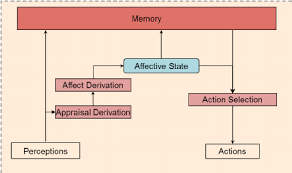
\includegraphics[width=.8\textwidth]{./Images/fatima-core}
%   \caption{FAtiMA Core's architecture.}
%   \label{fig:fatima-core}
% \end{figure}

% An agent is able to receive perceptions from the environment (events) which are used to update the agent's memory (or internal state) and to trigger the appraisal process.
% The result of the appraisal process is stored in the affective state, and later used to influence the action selection processes which will make the agent act upon the environment.
% Appraisal Derivation is responsible for evaluating the relevance of the event to the agent and determines a set of appraisal variables and affect derivation takes these variables as input to generate the resulting affective states (emotions or mood).

% As noted before, an agent using the \ac{FAtiMA} Core on its own will do nothing.
% Agency is achieved by adding several components (or modules) to the Core.
% In the scenario described in \cite{mascarenhas:cultural-behaviour}, the author used the following components:

% \begin{itemize}
% \item \textbf{Reactive Component}: uses a set of emotional reaction rules to determine values of some appraisal variables.
% \item \textbf{Deliberative Component}: handles goal-based behaviour and adds planning capabilities to the agent. It also uses the state of plans in memory to generate appraisal variables.
% \item \textbf{OCCAffectDerivation Component}: generates emotions from the appraisal variables according to the OCC Theory of Emotions \cite{ortony:occ}.
% \item \textbf{Motivational Component}: models needs and goals for the agent that will influence the utility of a given goal.
% \item \textbf{Theory of Mind Component}: creates a model of the internal states of other agents.
% \item \textbf{Cultural Component}: implements cultural-dependent behaviour of agents through the use of rituals, symbols, and cultural dimensions, and determine the impact actions have on the motivational states of the agents.
% \end{itemize}

\section{Closing Remarks}

\noindent The game industry is currently using outdated techniques to add behaviour to the characters that populate their games.
Skilled game designers can still create interesting behaviours with the used techniques, but the need for social context and active goal pursuit requires more advanced techniques.

To build a platform that will enable developers to create collaborative and believable \acp{NPC} for survival games, we've, first of all, looked into frameworks and tools that focus on agent creation.

\ac{JADE} provides a great platform for the development of agents.
However, \ac{JADE}'s main field of applicability is that of software engineering.
Its main purpose is the development of negotiating agents that conform to the \ac{FIPA} specification, having no concern whatsoever for interactions with humans, to such an extent that, although it is specified in \ac{FIPA}, \ac{JADE} is an agent-only platform with no support for Human-Agent Communication. 

NetLogo is a great example of testability, which is one of our main focus.
The ability to run fine tuned scenarios with different behaviours easily is a key point of its design and of utmost importance for our work, and that we will strongly value while developing our work.
Despite that, it does not provide a model for agency which is one of the crucial points of this work.

The final tool we've looked into is PsychSim.
As a social agent architecture, PsychSim presents a well-defined model capable of fully simulating social behaviour, is based on sound theories from psychology, and takes into account other agents in its cognitive process.
But, it lacks the possibility to have agents interacting with humans.
Additionally, as the agent's behaviour is based only in policies which guide it's immediate behaviour, each agent will follow the scenario devised by the developer without deviation.

We've then moved into exploring some of the currently used agency models.
The three systems we described were \ac{CiF}, Versu, and \ac{FAtiMA}.

Despite the successful implementation of \ac{CiF} in the game Prom Week \cite{mccoy:prom-week}, the game developers still need to specify every rule for every possible social interaction between \acp{NPC}.
Prom Week contains over forty nine hundred unique influence rules, around sixty social exchanges with over twenty rules that contribute to the characters' desires and responses, a cast of eighteen characters, and a combined total of over forty thousand predicates.
This represents an authoring burden that we want to avoid when developing our \acp{NPC}.
Even its successor, Ensemble, which lowers the authoring burden by adding social practices, has been recognized, by the authors, to possess limitations: a social practice must be taken to completion before another practice can be initiated, which does not reflect real social interaction.

Versu's logic powered approach is a differentiating aspect from the other models, however it does imposes some limitations.
One example is how the agents beliefs are expressed.
The system cannot represent universal and existential quantifiers (e.g. ``everyone has become insane" and ``the murderer is one of the guests", respectively) or beliefs about others' beliefs (e.g. ``Mr Quinn believes that Lucy believes that Mrs Quinn is the murderer").

Finally, and although \ac{FAtiMA}, by itself, is not a determined model for agency, it provides a set of ready to use assets, that allow developers to use whatever they need to achieve their goals.
The inclusion of emotional appraisal, theory of the mind models, and its planning capabilities make \ac{FAtiMA} the best candidate to be used.
This, allied with the fact that it has been successfully used in several social scenarios with human interaction (\cite{paiva:learning-by-feeling} \cite{rodrigues:i-can-feel-to} \cite{aylett:intercultural-empathy} \cite{correia:sueca}), the ability to extended the existing assets, and the ability to incorporate planning into its decision making process, make it the best choice for our work.

